\section{Optimizations}

\subsection{File Loading}
When loading a data resource, the biggest bottleneck is in the fetch from a persistent storage medium.
Doing multiple IO operations on a hard disk for example, can heavily increase the load time of a file
due to their mix with other IO operations from the rest of the Operating System\footnote{Programs do
not have exclusive ownership of the hard disk in a multitasking environment}. With this in mind, resources
from Hard Drive or other persistent storages are best loaded with the fewest IO operations that can be done.
In our case, files are being read in a single shot.

\subsection{Rendering State Changes Minimization}
Changing often the driver state (through OpenGL calls for example), can also steal precious time from the program.
This occurs because a possible driver call may change the state in our graphics card hardware or not depending
on the action we took.\footnote{Although, modern drivers often try to defer as much state change as possible
till the next draw call} Therefore, redundant graphics API calls are avoided and similar ones are batched
as much as possible.

\subsection{Deferred Rendering}
With the traditional Forward Rendering pipeline, each vertex passes through the Gpu processing pipeline
regardless if it is visible or not in the end. That means that lots of fragments are reaching the final
shading stage without any actual effect. In addition, this approach does not scale well with more lights
as the more lights we have, the more unnecessary shading operations we get. To avoid this rendering overhead
we need a way to be able to shade only the final visible fragments. This is achieved through a ``Deferred
Rendering'' pipeline that is composed in 2 main passes:

\begin{enumerate}
\item Geometry Pass
\item Lighting Pass
\end{enumerate}

\subsubsection{Geometry Pass}

\begin{figure}[ht]
    \centering
    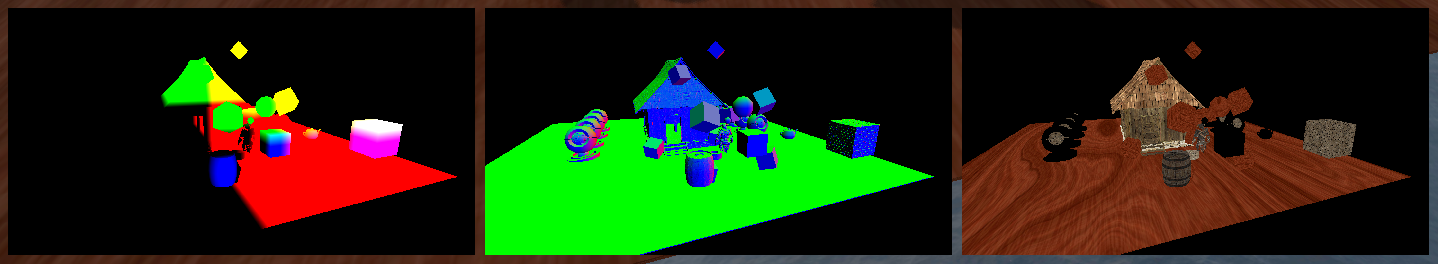
\includegraphics[scale=0.3, clip=true]{./image/gbuffer.png}
    \caption{Position, Normal and BaseColor GBuffer textures}
\label{fig:gbuf}
\end{figure}

In the Geometry Pass we render each object once. Base color, metalness, roughness, reflectivity, and world space normals
are rendered into framebuffer targets (textures) for each final fragment. This logical grouping of textures is named
a GBuffer (Geometry Buffer). The GBuffer is set as a Multiple Render Target output in the Geometry Pass, so in the end
of the fragment shading stage all the above mentioned data are saved to their respective texture in the GBuffer which,
in turn is bound and used when shading the given fragment in the Lighting Pass. The visualized contents of some GBuffer
textures can be seen in figure~\ref{fig:gbuf}.


\subsubsection{Lighting Pass}
The lighting pass consists of multiple individual light passes one per direct light plus one for the
environmental lighting. For each sub-pass one we compute the lighting for each screen space fragment using
the data from the GBuffer and the bound ShadowMaps.

\subsection{Bounding Spheres Optimization}
